% DO NOT COMPILE THIS FILE DIRECTLY!
% This is included by the other .tex files.


\begin{frame}
    
\includegraphics[scale=.3]{images/logo-circl-Forensics.png}
    \begin{itemize}
        \item[]
        \item[]
        \item[] 11. Live Response
    \end{itemize}
\end{frame}


\begin{frame}
  \frametitle{11.1 Volatile Data}
  \begin{itemize}
      \item Memory dump
      \item Live analysis:
      \begin{itemize}
          \item[] $\to$ System time
          \item[] $\to$ Logged-on users
          \item[] $\to$ Open files
          \item[] $\to$ Network -connections -status
          \item[] $\to$ Process information -memory
          \item[] $\to$ Process / port mapping
          \item[] $\to$ Clipboard content
          \item[] $\to$ Services
          \item[] $\to$ Command history
          \item[] $\to$ Mapped drives / shares
          \item[] $\to$ !!! Do not store information on the subject system !!!
      \end{itemize}
      \item Image of live system $($Possible issues$)$
      \item Shutdown and image if possible
  \end{itemize}
\end{frame}


\begin{frame}[fragile]
  \frametitle{11.1 Collecting Volatile Data}
  \begin{lstlisting}[basicstyle=\tiny]
  https://docs.microsoft.com/en-us/sysinternals/
  ----------------------------------------------
  \end{lstlisting}
  \begin{itemize}
        \item System Time
\begin{lstlisting}[basicstyle=\tiny]
> date /t & time /t            # Don't foget to note wall-clock-time
    Tue 03/26/2019             # Note timezone of PC
    01:31 PM
\end{lstlisting}
        \item Loggedon Users
\begin{lstlisting}[basicstyle=\tiny]
> net session

> .\PsLoggedon.exe
    Users logged on locally:
         3/26/2019 1:30:23 PM       John-PC\John
    No one is logged on via resource shares.

> .\logonsessions.exe
    [5] Logon session 00000000:0001ad9d:
        User name:    John-PC\John
        Auth package: NTLM
        Logon type:   Interactive
        Session:      1
        Sid:          S-1-5-21-3031575581-801213887-4188682232-1001
        Logon time:   3/26/2019 1:30:23 PM
        Logon server: JOHN-PC
\end{lstlisting}
    \end{itemize}
\end{frame}


\begin{frame}[fragile]
  \frametitle{11.1 Collecting Volatile Data}
  \begin{itemize}
        \item Open Files
\begin{lstlisting}[basicstyle=\tiny]
> net file

> .\psfile.exe
\end{lstlisting}
        \item Network Connections and Status
\begin{lstlisting}[basicstyle=\tiny]
> netstat -anob
    Proto  Local Address      Foreign Address     State         PID    RpcSs
    TCP    0.0.0.0:135        0.0.0.0:0           LISTENING     696    [svchost.exe]
    TCP    0.0.0.0:445        0.0.0.0:0           LISTENING     4
    TCP    0.0.0.0:554        0.0.0.0:0           LISTENING     2504   [wmpnetwk.exe]
    TCP    0.0.0.0:10243      0.0.0.0:0           LISTENING     4
    TCP    0.0.0.0:49152      0.0.0.0:0           LISTENING     364    [wininit.exe]

> netstat -rn
    Network Destination        Netmask          Gateway       Interface  Metric
              0.0.0.0          0.0.0.0         10.0.2.2        10.0.2.15     10
             10.0.2.0    255.255.255.0         On-link         10.0.2.15    266
            10.0.2.15  255.255.255.255         On-link         10.0.2.15    266

> ipconfig /all
\end{lstlisting}
    \end{itemize}
\end{frame}


\begin{frame}[fragile]
  \frametitle{11.1 Collecting Volatile Data}
  \begin{itemize}
        \item Running Processes
\begin{lstlisting}[basicstyle=\tiny]
> tasklist
    Image Name                     PID Session Name        Session#    Mem Usage
    ========================= ======== ================ =========== ============
    System                           4 Services                   0        600 K
    smss.exe                       252 Services                   0        792 K
    csrss.exe                      328 Services                   0      3,224 K
    wininit.exe                    364 Services                   0      3,316 K
    csrss.exe                      372 Console                    1      4,196 K
    winlogon.exe                   400 Console                    1      6,272 K
    services.exe                   460 Services                   0      6,628 K
    lsass.exe                      468 Services                   0      8,428 K
    lsm.exe                        476 Services                   0      3,040 K
    svchost.exe                    584 Services                   0      6,596 K
    cmd.exe                       3100 Console                    1      2,480 K

> tasklist /svc
    Image Name                     PID Services
    ========================= ======== ============================================
    svchost.exe                    584 DcomLaunch, PlugPlay, Power
    svchost.exe                    696 RpcEptMapper, RpcSs
    svchost.exe                    792 Audiosrv, Dhcp, eventlog,
                                       HomeGroupProvider, lmhosts, wscsvc
    svchost.exe                    844 AudioEndpointBuilder, CscService,
                                       HomeGroupListener, Netman, TrkWks, UxSms,
    svchost.exe                    876 EventSystem, fdPHost, FontCache, netprofm,
                                       nsi, WdiServiceHost
\end{lstlisting}
    \end{itemize}
\end{frame}


\begin{frame}[fragile]
  \frametitle{11.1 Collecting Volatile Data}
  \begin{itemize}
        \item Running Processes
\begin{lstlisting}[basicstyle=\tiny]
> .\pslist.exe -x

> .\pslist.exe -t
    Name                             Pid Pri Thd  Hnd      VM      WS    Priv
    explorer                        1252   8  26  912  212044   47672   36304
      VBoxTray                       360   8  12  153   61384    5624    1476
      cmd                            548   8   1   24   29256    2564    2628
        pslist                      3452  13   1  123   45908    3640    1652
      WzPreloader                   1244   8   6  119  109748    9064   11224
      cmd                           3100   8   1   20   27464    2480    1804

> .\Listdlls.exe

> .\handle.exe
\end{lstlisting}
        \item Processes/Port Mapping
\begin{lstlisting}[basicstyle=\tiny]
> .\tcpvcon -n -c -a
    TCP,svchost.exe,692,LISTENING,0.0.0.0,0.0.0.0
    TCP,System,4,LISTENING,10.0.2.15,0.0.0.0
    TCP,wmpnetwk.exe,2428,LISTENING,0.0.0.0,0.0.0.0
    TCP,wininit.exe,364,LISTENING,0.0.0.0,0.0.0.0
    TCP,svchost.exe,776,LISTENING,0.0.0.0,0.0.0.0
    TCP,svchost.exe,896,LISTENING,0.0.0.0,0.0.0.0
    TCP,services.exe,460,LISTENING,0.0.0.0,0.0.0.0
\end{lstlisting}
    \end{itemize}
\end{frame}


\begin{frame}[fragile]
  \frametitle{11.1 Collecting Volatile Data}
  \begin{itemize}
        \item Command History
\begin{lstlisting}[basicstyle=\tiny]
> doskey /history
    netstat -anob
    .\Listdlls.exe
    .\handle.exe
    .\tcpvcon -n -c -a
    cls
    doskey /history
\end{lstlisting}
        \item Processes/Port Mapping
\begin{lstlisting}[basicstyle=\tiny]

\end{lstlisting}
    \end{itemize}
\end{frame}


\begin{frame}[fragile]
  \frametitle{11.2 Non Volatile Data}
  \begin{itemize}
        \item Clear Pagefile at shutdown
\begin{lstlisting}[basicstyle=\tiny]
> reg QUERY "HKLM\SYSTEM\CurrentControlSet\Control\Session Manager\Memory Management"
    .....
    ClearPageFileAtShutdown    REG_DWORD    0x0
    .....
\end{lstlisting}
        \item Update Last Access disabled
\begin{lstlisting}[basicstyle=\tiny]
> reg QUERY "HKLM\SYSTEM\CurrentControlSet\Control\FileSystem"
    .....
    NtfsDisableLastAccessUpdate    REG_DWORD    0x0
    .....
\end{lstlisting}
        \item Autostart locations
\begin{lstlisting}[basicstyle=\tiny]
> .\Autoruns.exe
\end{lstlisting}
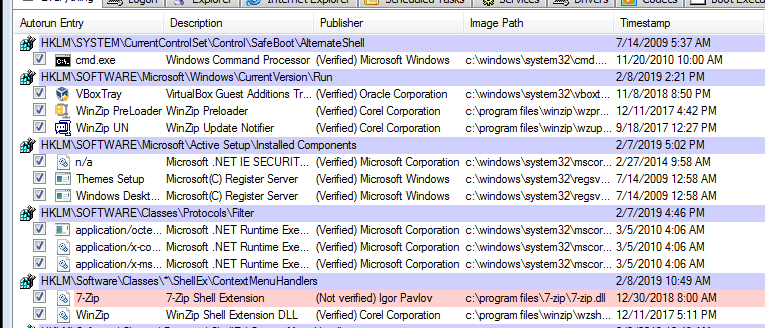
\includegraphics[scale=.27]{images/f11_autorun.png}
  \end{itemize}
\end{frame}


\begin{frame}[fragile]
  \frametitle{11.3 Across the network}
  \begin{itemize}
        \item Get Nmap command-line zipfile
	\item[] \url{https://nmap.org/download.html}
	\item[]
        \item On Linux set up a netcat listener
\begin{lstlisting}[basicstyle=\tiny]
nc -k -l 9999 >> logfile.txt
\end{lstlisting}
        \item Sending from subject system
\begin{lstlisting}[basicstyle=\tiny]
ncat aaa.bbb.ccc.ddd 9999

echo "Date and Time" | ncat.exe aaa.bbb.ccc.ddd 9999
date /t | ncat.exe aaa.bbb.ccc.ddd 9999
time /t | ncat.exe aaa.bbb.ccc.ddd 9999
echo "-------------" | ncat.exe aaa.bbb.ccc.ddd 9999
\end{lstlisting}
  \end{itemize}
\end{frame}







